\section{Experiment 3: Adding Semantic Noise}

% Corresponding Progress Reports
% https://www.notion.so/241025-Matthias-Exploration-of-adversarial-augmentation-199ccb0746f74fd696b8bebe8590fe15
% https://www.notion.so/241101-Matthias-Using-Adversarial-perturbation-to-augment-clip-vision-input-in-brain-diffuser-3e8235a27e3c4f4eb67f61a467fd5ada
% https://www.notion.so/241108-Matthias-further-exploration-of-perturbations-196925e9c9b94c04be7a7d1891ce5389?pvs=23
% https://www.notion.so/241114-matthias-brain-diffuser-perturbation-big-analysis-13cb45eff9104ae1929522dcf1d39bb9?pvs=23

% How to execute the whole advpert process?
% 1. Execute multi_process_pert_generation.py (it will generate perturbations for all conditions)
% 2. Execute re_recon_main.py (it will do the reconstructions for all cases -> make sure all data is ready before, baseline needs to be computed beforehand)
% 3. Execute quantitative_eval.py (extracts the quantitative measures from all predicted features/imates)
% 4. Execute create_dfs_advpert.py (creates the dataframes to evaluate the results)
% 5. Execute the analysis_advpert.py (generates the plots)
% 6. For the additional validation plots, execute clip_module_testing.py


\subsection{Background}

\subsection{Methods}

The perturbation procedure is described below. The training images are to be manipulated in such a way that they look almost the same, but the semantic information that the clipvision encoder reads from them is greatly altered. Two different algorithms are analysed to generate the perturbations in the images. It is then determined which of the two algorithms is better at achieving the goal of keeping the input image visually as close to the original as possible while at the same time producing different clipvision embeddings. Subsequently, all training data is perturbed using this algorithm and the perturbed versions are used to train the clipvision translator of the brain diffuser algorithm.

\subsubsection{Perturbation Process}

% FGSM Algorithm Formula
First, the Fast Gradient Sign Method\cite{goodfellowExplainingHarnessingAdversarial2014} (FGSM) is used to generate the perturbations. In FGSM, an image is first encoded with a model (here the clipvision encoder) in a forward step, then a loss to a desired output vector (the perturbation vector is calculated with respect to the input image , then the sign of the gradient (multiplied by a freely chosen factor $\epsilon$) is subtracted from the input image in a single backpropagation step. This procedure ensures that the clipvision output of the perturbed image is more similar to the perturbation vector. The mathematical description of the algorithm is as follows

\[
x' = x + \epsilon \cdot \text{sign}(\nabla_x J(\theta, x, y))
\]

where:
\begin{itemize}
    \item \( x' \) is the perturbed image,
    \item \( x \) is the original image,
    \item \( y \) is the perturbation vector,
    \item \( \epsilon \) is the perturbation factor,
    \item \( \nabla_x J(\theta, x, y) \) is the gradient of the loss function \( J \) w.r.t.\ \( x \),
    \item \( \text{sign}(\cdot) \) is the element-wise sign function.
    \item \( \theta \) represents the model parameters,
\end{itemize}

In principle, all possible vectors that have the same output format as the clipvision encoder can be used as perturbation vectors. In our case, we take advantage of the multimodality of the clip model and can use cliptext embeddings as perturbation vectors. In this way, the semantic information from the captions can be partially stored in the images, at best without being highly visible in the images. In our case, two types of captions are inserted into the images via the perturbation: on the one hand, captions are used that represent the valid image in question (e.g.\ a caption describing the bat for an image of a bat). On the other hand, invalid captions are used, i.e.\ where the caption describes something other than what can be seen in the image. The perturbations with valid captions will be referred to as `friendly perturbations', the perturbations with invalid captions as `adversarial perturbations'.

% IC Algorithm Formula
In addition to the one-step FGSM algorithm, an iterative perturbation method developed for this work is used. Here, too, the input image is systematically adjusted by backpropagation so that the output of the clipvision model of the perturbed input image approach a previously selected perturbation vector. As before, this perturbation vector must be in the same space as in the FGSM algorithm, and again cliptext embeddings of friendly and adversarial captions are used. The difference to the FGSM algorithm is that the perturbation is not performed in a single step, but iteratively in several steps until a criterion is reached. The criterion determines how similar (measured by cosine distance) the output of the clipvision embedding of the perturbed image should be to the perturbation vector in comparison to the original image. For example, with a criterion of 50/50, the input image would be perturbed until the clipvision embeddings of the perturbed version have the same cosine distance from the perturbation vector as the original clipvision embeddings (with a criterion of 10/90, until the distance of the perturbed embeddings from the perturbation vector is greater than 11.1\% of the distance of the perturbed embeddings from the original embeddings). In addition, a maximum number of steps is introduced if the algorithm does not reach the target criterion. The formal definition of the algorithm is as follows 

\[
\begin{aligned}
& \textbf{Iteration: For } t = 0 \text{ to steps:}\\
& \quad 1.\; \mathbf{v}_t = \mathrm{clipvision.encode}(\mathbf{x}_t), \\[4pt]
& \quad 2.\; \ell(\mathbf{x}_t) 
\;=\; \cos\bigl(\mathbf{v}_t,\;\mathbf{v}_c\bigr), \\[4pt]
& \quad 3.\; \mathbf{x}_{t+1} 
\;=\; \mathbf{x}_t \;-\; \eta \,\nabla_{x_t} (\theta, x_t, v_c), \\[4pt]
& \quad 4.\; d_{\text{init}} 
\;=\; \cos\bigl(\mathbf{v}_t,\;\mathbf{v}_0\bigr), \\[4pt]
& \quad 5.\; \textbf{if} \;\frac{d_{\text{init}}}{\ell(\mathbf{x}_t)} 
\;>\; LC, \;\textbf{then break}.\\[6pt]
%
& \textbf{Output: } \mathbf{x}_t \quad \text{(perturbed image)}.
\end{aligned}
\]

where:
\begin{itemize}
    \item $\mathbf{x}_0$ is the original input image
    \item $\eta$ is the learning rate
    \item $LC$ is the stop criterion (number between 0 and 1)
    \item $v_0$ is the clipvision encoding of $x_0$
    \item $v_c$ is the cliptext encoding of the selected caption
    \item cos is the cosine distance
    \item steps is the maximum number of steps to iterate
\end{itemize}

For faster convergence, the learning rate is set to 3 in the first 100 steps, to 1.5 between step 100 and step 300 and then to 1. The maximum number of steps is set to 500.

\subsubsection{Perturbation Validation}

% Image from smith clip_module_testing.py
\begin{figure}[ht]
    \centering
    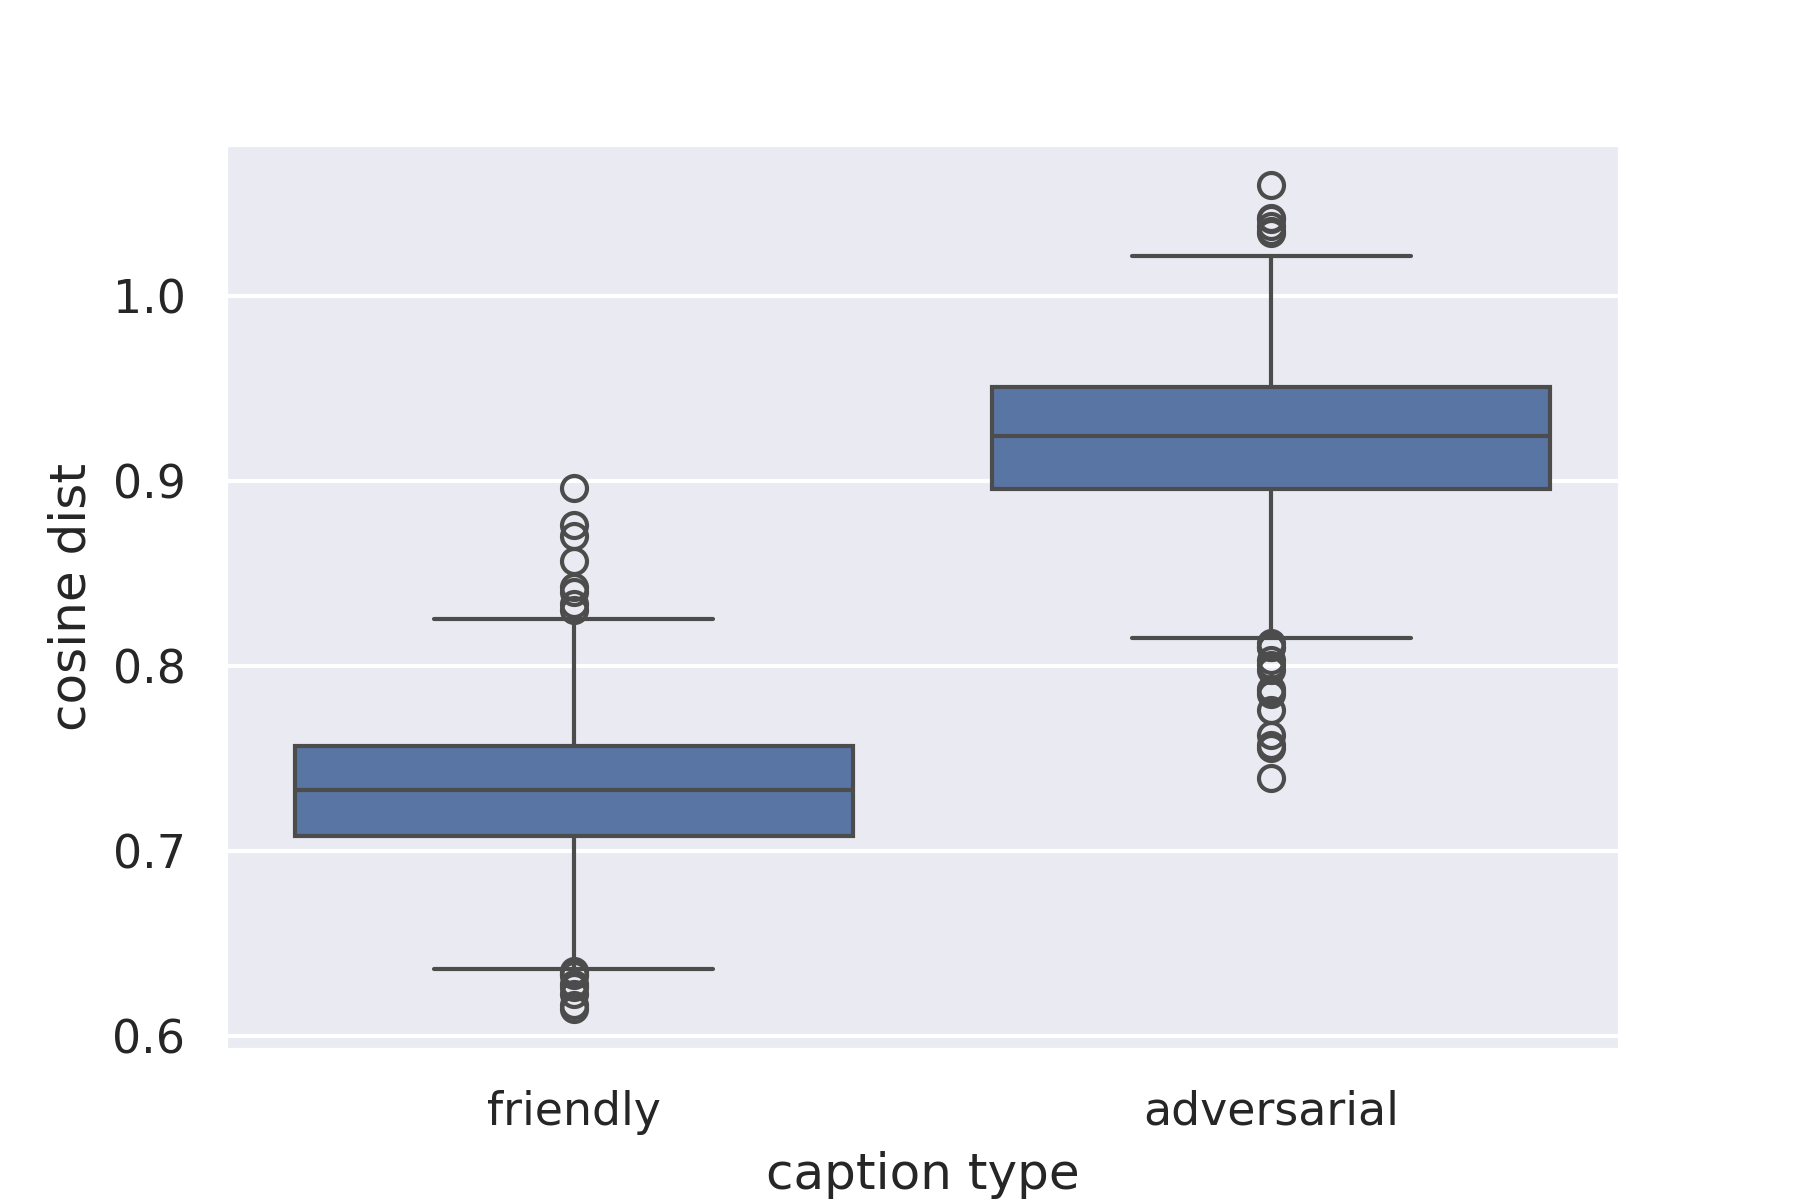
\includegraphics[width=0.6\textwidth]{plots/advpert_sanity_check_friendly_vs_adversarial_cap.png}
    \caption{A nice image}\label{fig:advpert_sanity_check_friendly_vs_adversarial_cap}
\end{figure}
% TODO: Describe the image
% -> Shows, that the corresponding captions are actually closer to the images than the other ones.
% Conclusion: I can do things like friendly and adversarial perturbations


% Show how the loss is developing for the IC criterion 
% TODO: need an image for that
% Both friendly and adversarial in one image -> To show, that both of them develop similarly
\begin{figure}[ht]
    \centering
    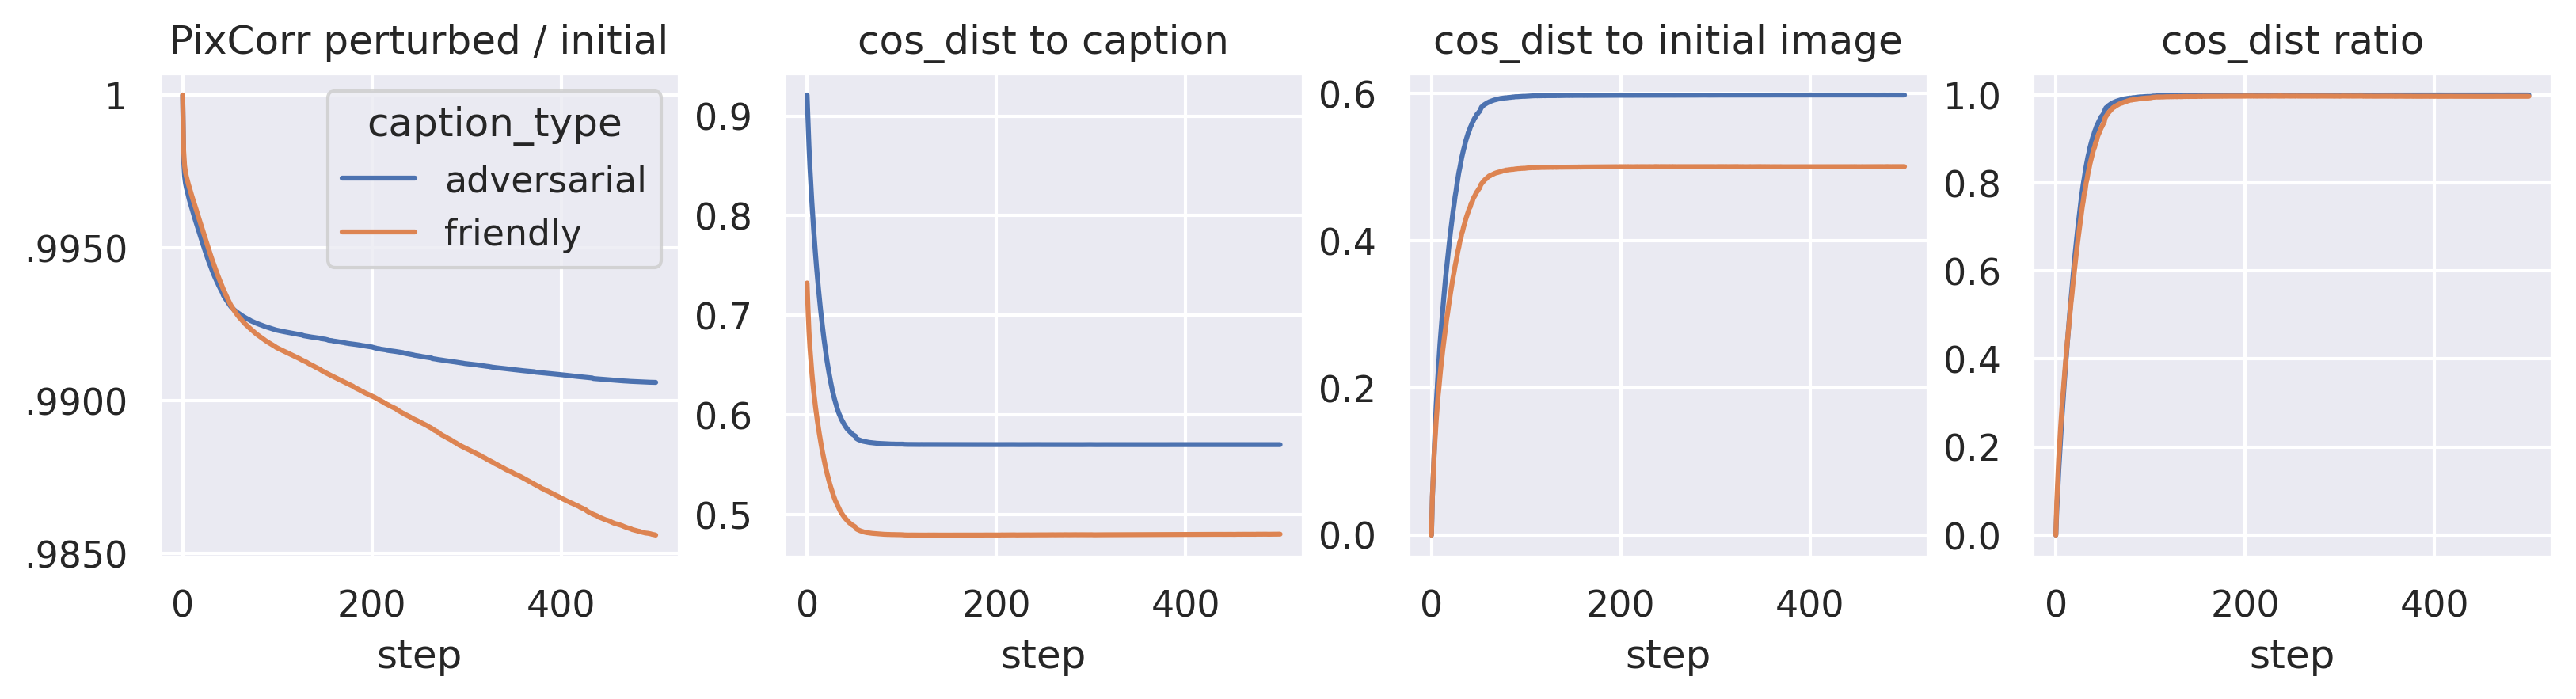
\includegraphics[width=1\textwidth]{plots/advpert_validation_ic_loss_curves.png}
    \caption{A nice image}\label{fig:advpert_validation_ic_loss_curves}
\end{figure}


% Show how the results of IC change with more and more epochs (together with the IC loss plot)
    % With images for each epoch

\begin{figure}[ht]
    \centering
    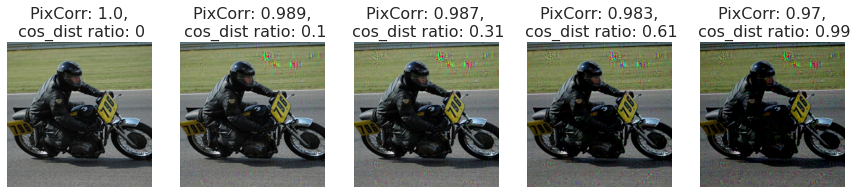
\includegraphics[width=1\textwidth]{plots/advpert_ic_qual_validation_evolution.png}
    \caption{A nice image}\label{fig:advpert_ic_qual_validation_evolution}
\end{figure}

% Show how the FGSM changes the images (Qualitative)
    % With different Epsilons

\begin{figure}[ht]
    \centering
    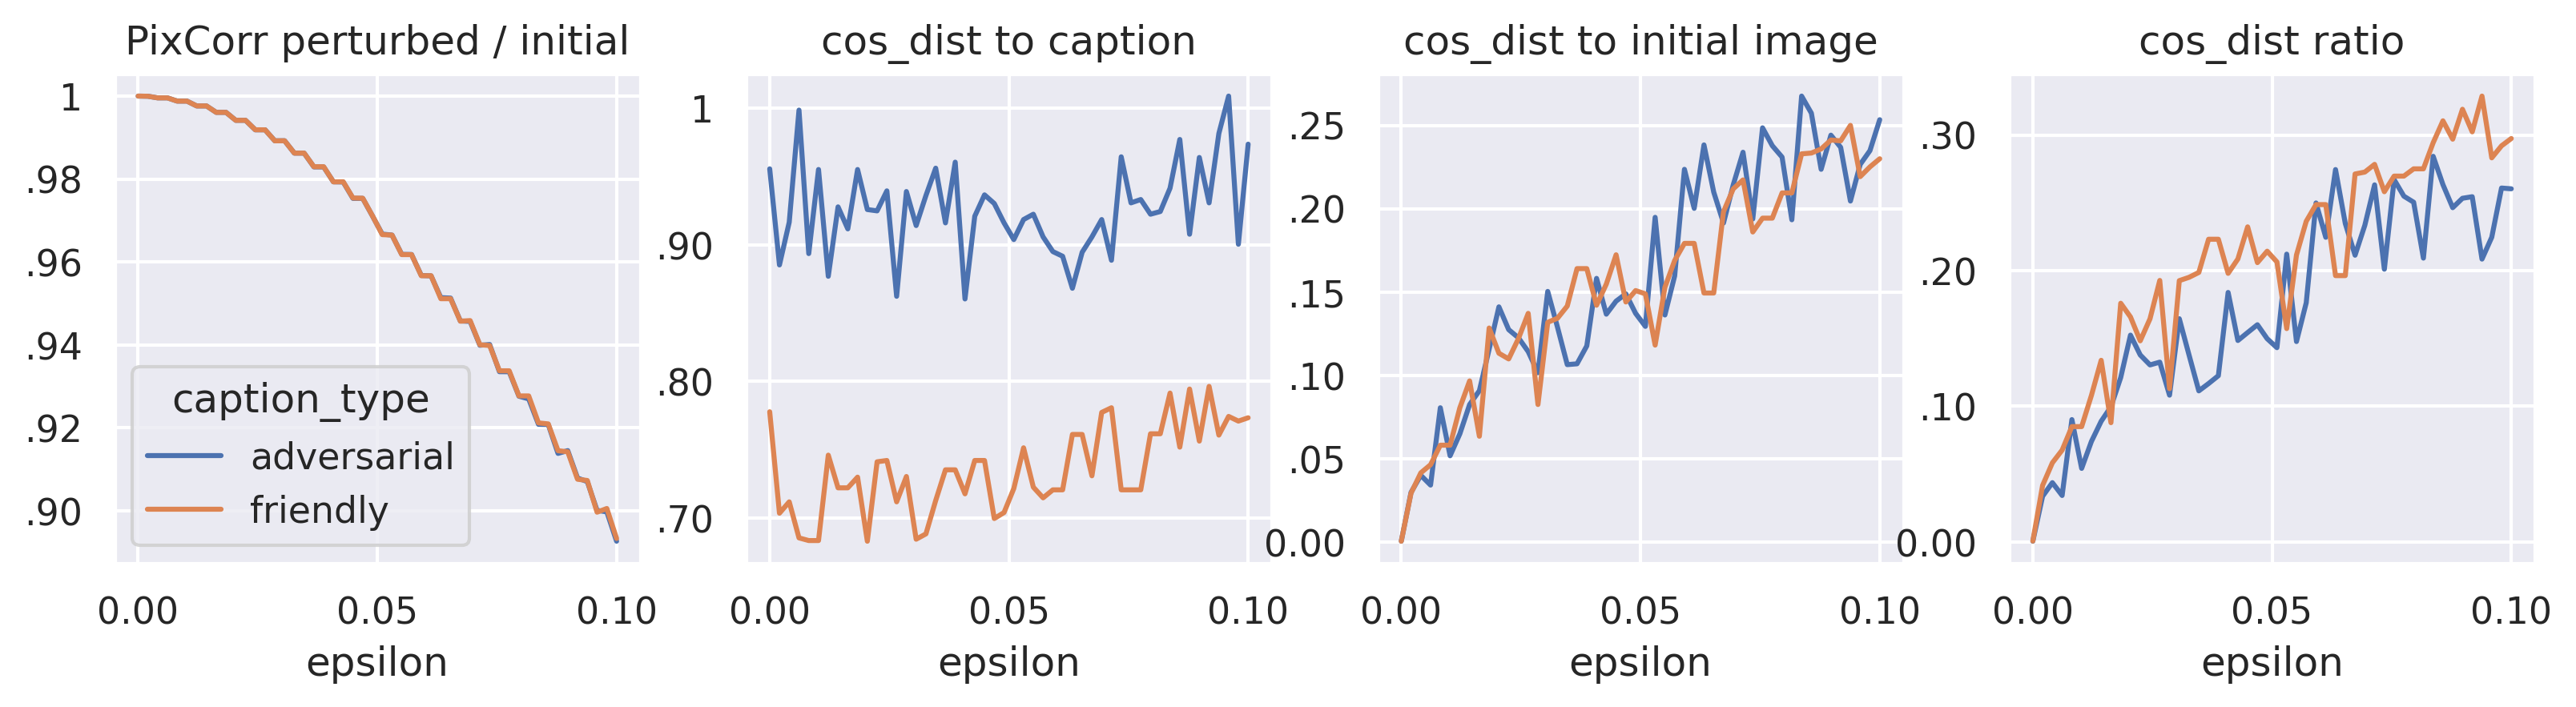
\includegraphics[width=1\textwidth]{plots/advpert_validation_fgsm_loss_curves.png}
    \caption{A nice image}\label{fig:advpert_validation_fgsm_loss_curves}
\end{figure}

% Show the influence of friendly vs adversarial perturbation on PixCorr
    % Both for FGSM and for IC
    % -> Not so much changes in the images
\begin{figure}[ht]
    \centering
    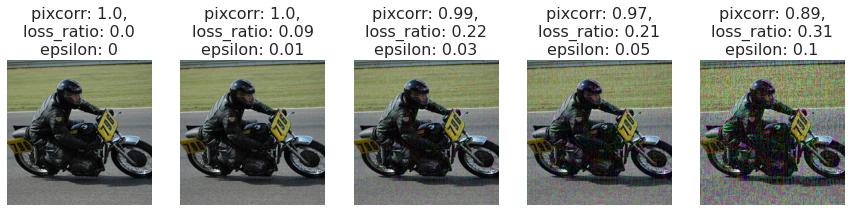
\includegraphics[width=1\textwidth]{plots/advpert_fgsm_qual_validation_evolution.png}
    \caption{A nice image}\label{fig:advpert_fgsm_qual_validation_evolution}
\end{figure}

% Define the parameters that will be used in the final test 
    % 90/10 for IC and 0.03 for FGSM

% Show how loss to original clipfeatures and caption clip features are on average for the chosen perturbations
    % Don't need to show ALL the pictures here I guess? Otherwise I'd have to do the whole perturbation process again
    % oh boy. Oh you poor little boy...

\begin{figure}[ht]
    \centering
    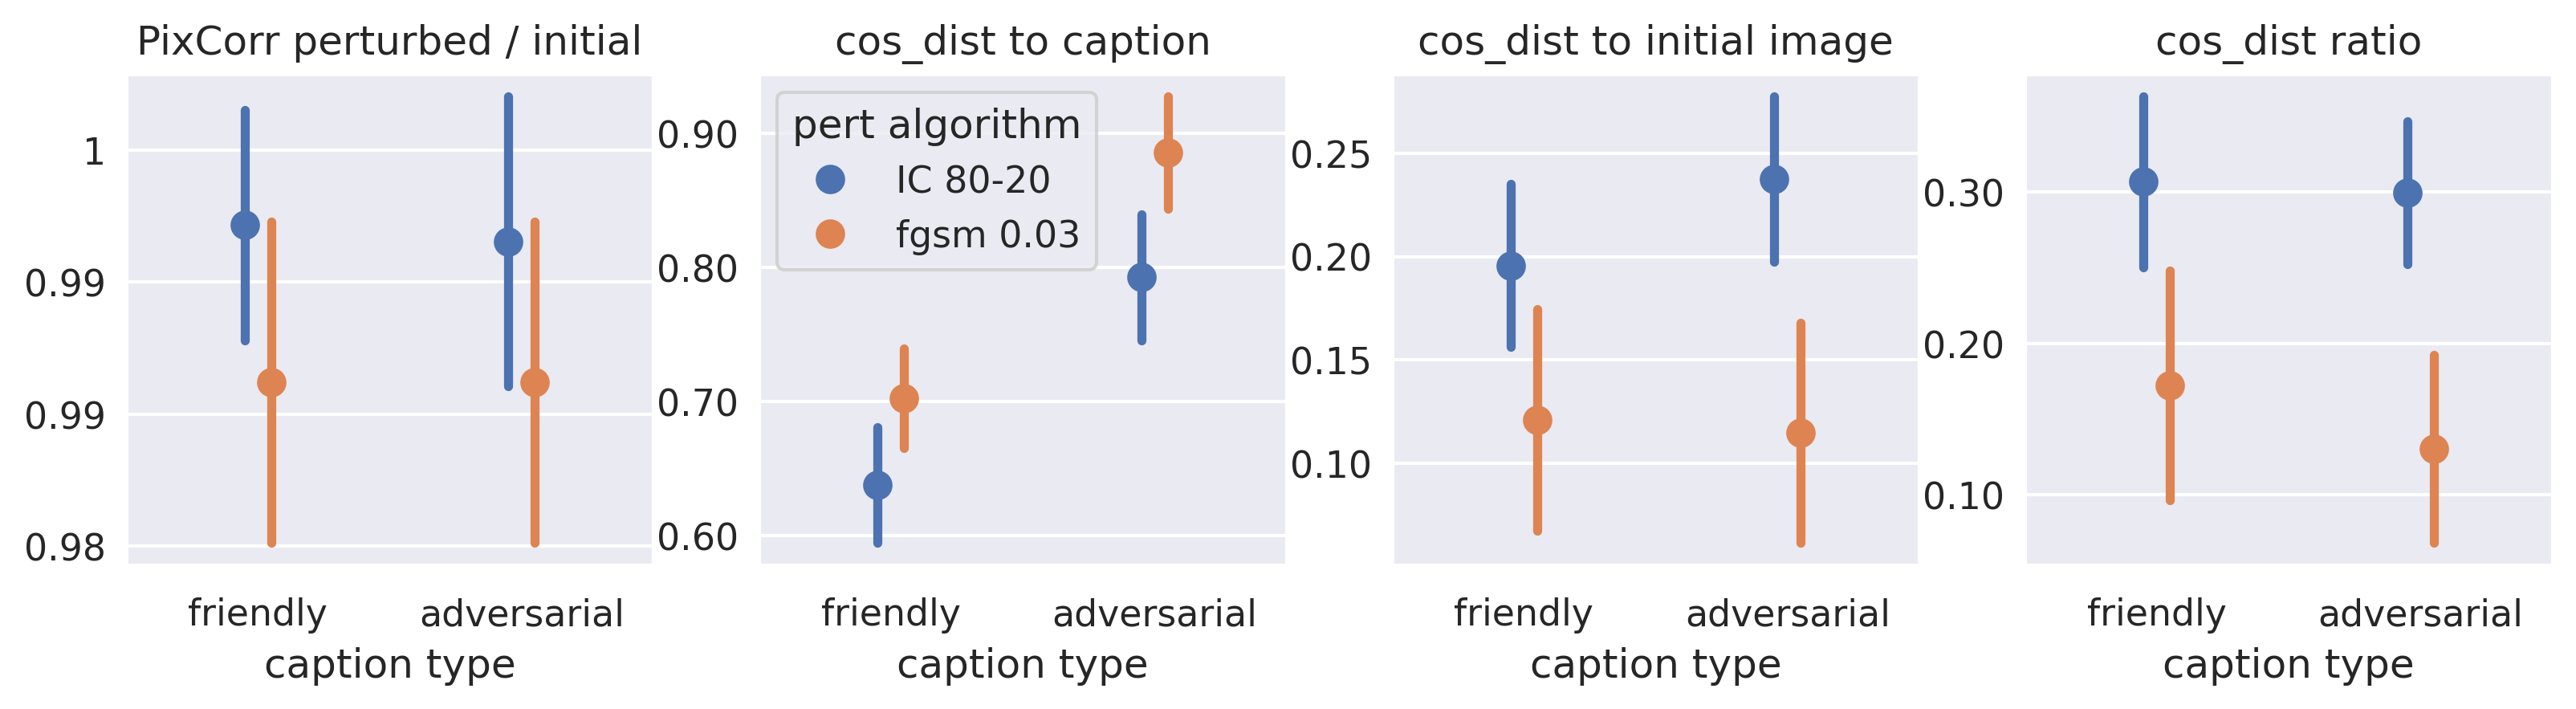
\includegraphics[width=1\textwidth]{plots/advpert_validation_chosen_perts.png}
    \caption{A nice image}\label{fig:advpert_validation_chosen_perts}
\end{figure}


% Show some of the images qualitatively that will be shown
\begin{figure}[ht]
    \centering
    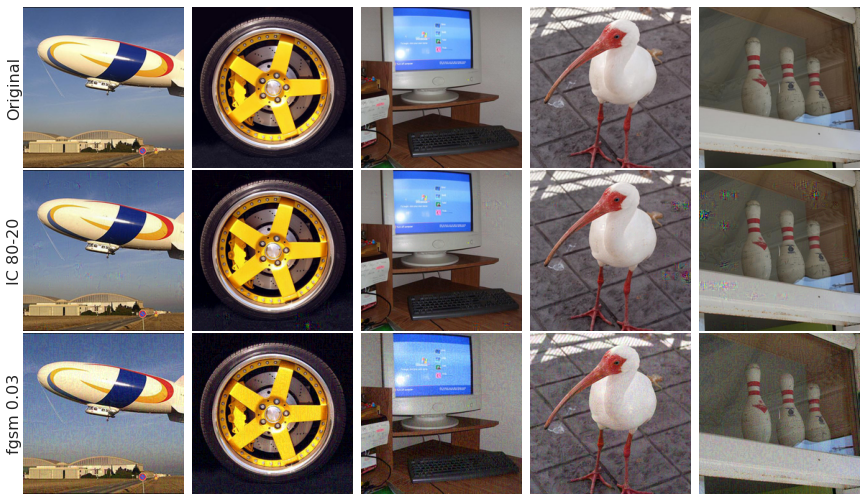
\includegraphics[width=1\textwidth]{plots/advpert_validation_chosen_qual.png}
    \caption{A nice image}\label{fig:advpert_validation_chosen_qual}
\end{figure}


\subsection{Results}

\subsection{Discussion}

- Man könnte natürlich auch die KI generierten captions genutzen